\section{Data}
\begin{frame}{Data}
\begin{itemize}
\item Datasæt fra FRED
\begin{itemize}
\item 128 variable
\item 1. januar 1959 - 1. november 2017 (707 observationer)
\item Opdelt i 8 grupper:
\begin{columns}
\begin{column}{0.35\textwidth}
    \begin{enumerate}
	\item Output og indkomst \legendbox{chartreuse4}
	\item Arbejdsmarked  \legendbox{blue3}
	\item Bolig \legendbox{purple}
	\item Forbrug, ordrer og varebeholdninger \legendbox{red3}
\end{enumerate}
\end{column}
\begin{column}{0.35\textwidth} 
    \begin{enumerate}
    \setcounter{enumi}{4}
	\item Penge og kredit \legendbox{deeppink}
	\item Renter og valutakurser \legendbox{orange}
	\item Priser \legendbox{cadetblue2}
	\item Aktiemarked \legendbox{goldenrod4}
\end{enumerate}
\end{column}
\end{columns}
\end{itemize}

\item Transformerede datasæt
\begin{itemize}
\item 123 variable
\item 1. januar 1960 - 1. juli 2017 (691 observationer)
\begin{itemize}
\item Træningsmængde: 1. januar 1960 - 1. december 2005 (552 observationer)
\item Testmængde: 1. januar 2006 - 1. juli 2017 (139 observationer)
\end{itemize}
\item Vi centrerer responsvariablen og standardiserer prædiktorerne.
\end{itemize}
\end{itemize}
\end{frame}

\begin{frame}{Data}{Arbejdsløshedsraten}
%\item Arbejdsløshedsraten betragtes som responsvariabel
%\begin{itemize}
%\item repræsenterer den procentvise ledighed af arbejdsstyrken
%\end{itemize}
%
\begin{figure}
 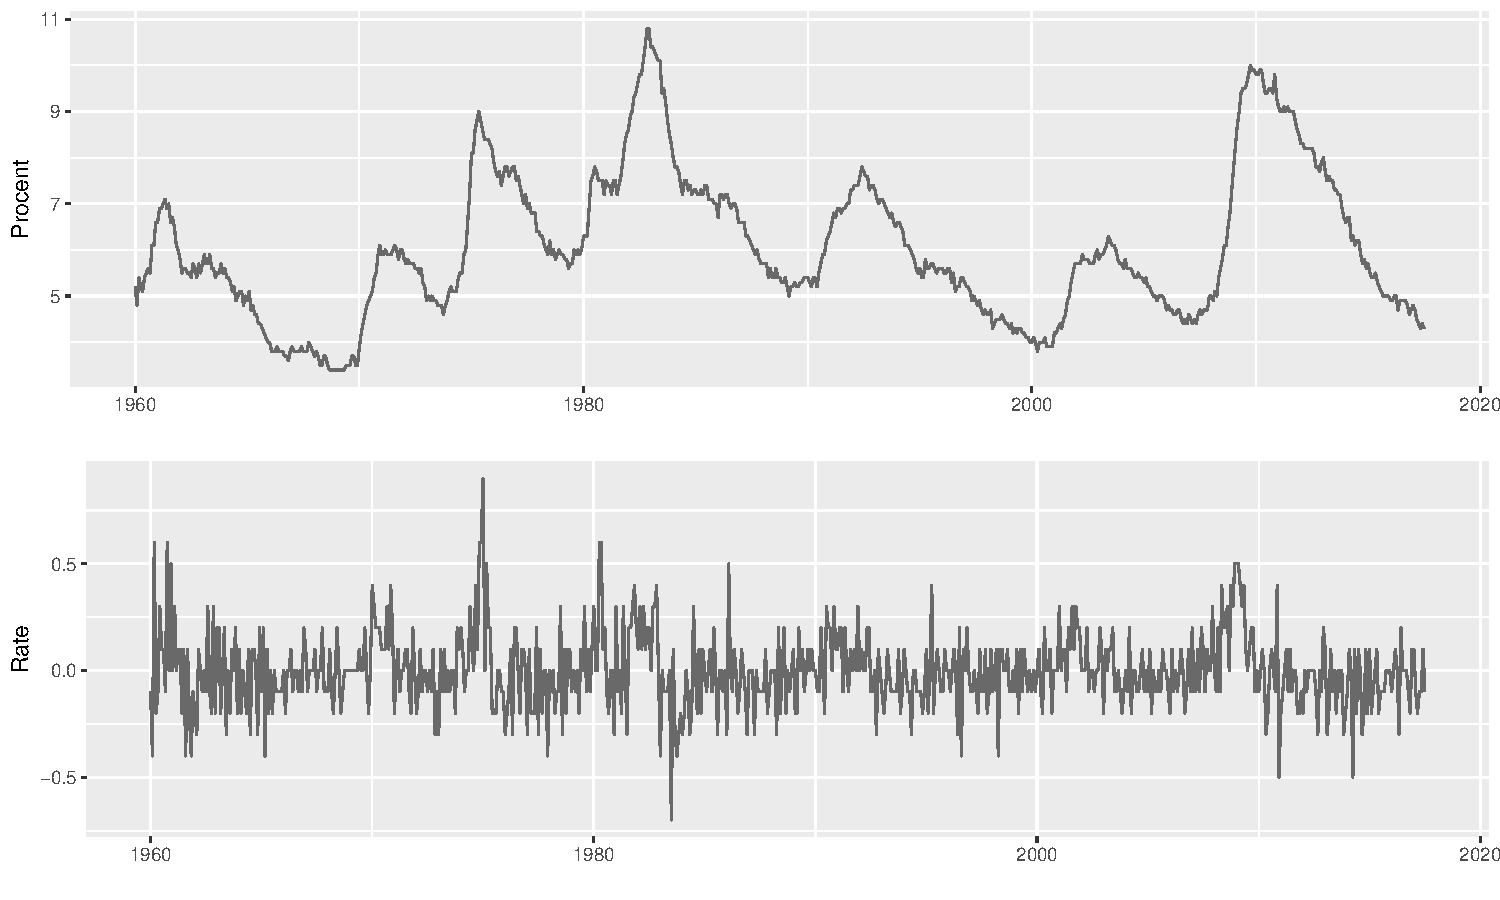
\includegraphics[width=1\linewidth, height=0.7\textheight]{slides/unemployment.pdf}
 \caption{Arbejdsløshedsraten og 1. differensen af arbejdsløshedsraten fra 1. januar 1960 til 1. juli 2017.}
 \end{figure}
%
\end{frame}

%%% Local Variables:
%%% mode: latex
%%% TeX-master: "../beamer"
%%% End:
